\section{ADC}
\label{sec:adc}
\textit{\hyperlink{schematic.4}{schematic}}

\subsection{Overview}
\label{sec:adc-overview}

The ADC is used to digitize signals amplified by the IF \hyperref[sec:ada4940-2]{ADA4940-2}
differential amplifiers before sending them to the \hyperref[sec:xc7a15t-ftg256]{FPGA} for
processing.

\subsection{LTC2292}
\label{sec:ltc2292}

\subsubsection{Description}
\label{sec:ltc2292-description}

The LTC2292 is a 40MHz, 12-bit differential input ADC\@. It has a max differential input voltage of
$2 \si{V}$ and uses twos complement output encoding which makes the minimum detectable (LSB) voltage
magnitude equal to about $1 \si{mV}$ \fixme{Make sure this is correct. It should be fairly evident
  after writing the relevant FPGA code}. The sampling frequency sets the Nyquist frequency at
$20 \si{MHz}$, well above the several hundred $\si{kHz}$ that characterize our signal
frequencies. By oversampling, we're able to relax anti-aliasing filter requirements, which improves
bandwidth and resolution.

\begin{figure}[h]
        \centering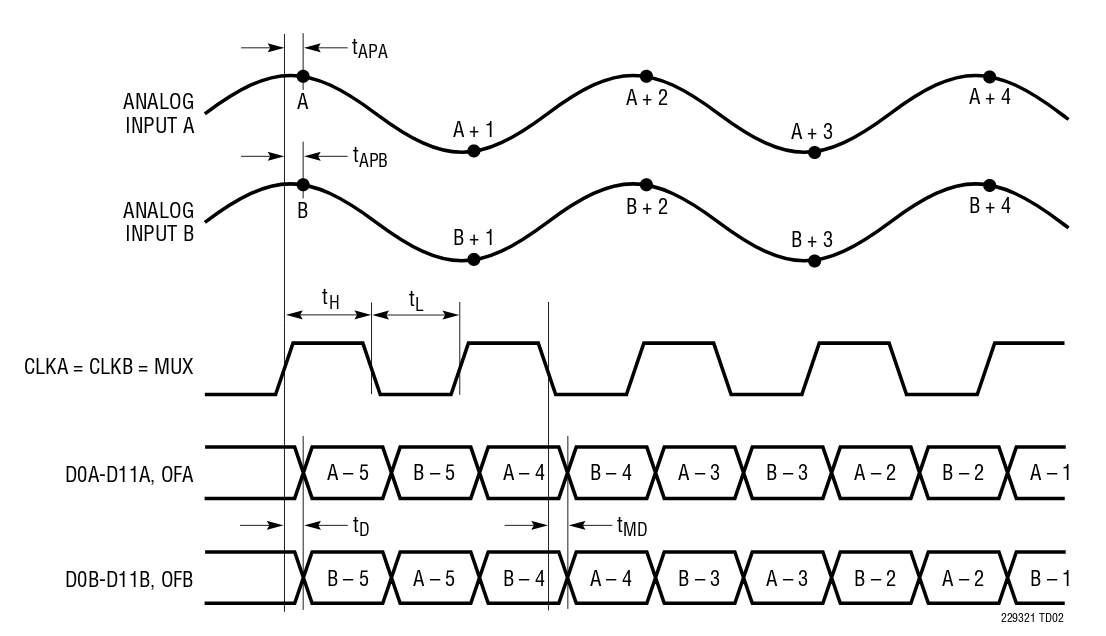
\includegraphics[width=0.75\textwidth]{data/LTC2292-multiplex.png}
        \caption{Multiplexed digital output bus timing for the LTC2292 ADC.}
        \label{fig:ltc2292-multiplex}
\end{figure}

\subsubsection{Linked Sections}
\label{sec:ltc2292-linked-sections}

\textit{\hyperref[sec:ltc2292-pinout]{pinout}}

\subsubsection{Component Selection}
\label{sec:ltc2292-component-selection}

\fixme{The part about the input filter should get its own section.}

The analog inputs employ anti-aliasing filters. The filters provide several benefits: (1) they
reduce aliasing by attenuating signals above the Nyquist frequency, (2) they limit wideband noise at
the input at the ADC input, which is important because the converter has a $575 \si{MHz}$ full-power
bandwidth, and (3) they isolate the \hyperref[sec:ada4940-2]{IF amplifier} from ADC noise at the
sampling frequency. Lastly, the capacitors act as a necessary charge source for the ADC input
capacitor. The two outer $100 \si{pF}$ capacitors (between the signal lines and ground) provide CMR
low-pass filtering with a cutoff frequency of $32 \si{MHz}$ (equation given in
Eq.~\ref{eq:anti-alias-cm-lp-filter}). The capacitor between the signal lines provides differential
low-pass filtering with a cutoff frequency of $16 \si{MHz}$. A
\href{https://e2e.ti.com/blogs_/archives/b/precisionhub/archive/2015/11/06/three-guidelines-for-designing-anti-aliasing-filters}{post
  from TI} explains this filtering. It's also important to keep the series resistor value low, since
the greater the resistance, the greater the Johnson noise.

\begin{equation}
        \label{eq:anti-alias-cm-lp-filter}
        f_{\text{c}} = \frac{1}{2 \pi R C}
\end{equation}

\subsubsection{PCB Layout}
\label{sec:ltc2292-pcb}

The $100 \si{nF}$ capacitors connected between the REFxx pins should placed as close to the pins as
possible.

The differential input traces should run parallel to one another and should be placed close
together. Additionally, they should be made as short as possible.

%%% Local Variables:
%%% mode: latex
%%% TeX-master: "fmcw-radar"
%%% End:
